\documentclass[tikz]{standalone}
\usetikzlibrary{angles}

\begin{document}
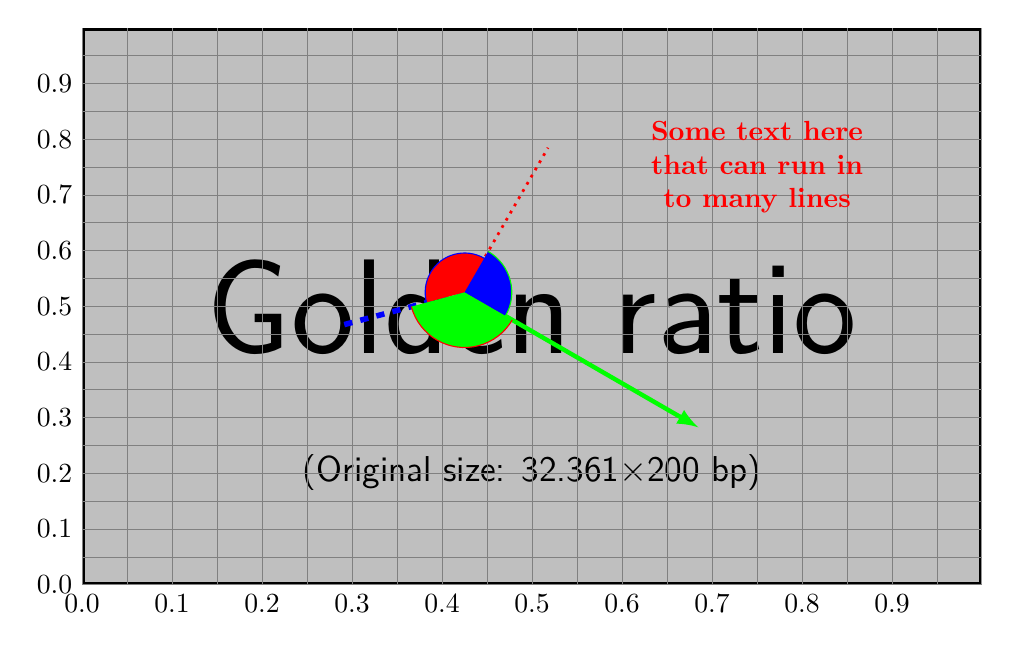
\begin{tikzpicture}
    \node[anchor=south west,inner sep=0] (image) at (0,0,0) {\includegraphics{example-image-golden}};
    \begin{scope}[x={(image.south east)},y={(image.north west)}]
        % next four lines will help you to locate the point needed by forming a grid. 
        % comment these four lines in the final picture.↓
        \draw[help lines,xstep=.1,ystep=.1] (0, 0) grid (1, 1);
        \draw[help lines,xstep=.05,ystep=.05] (0, 0) grid (1, 1);
        \foreach \x in {0,1,...,9} { \node [anchor=north] at (\x/10,0) {0.\x}; }
        \foreach \y in {0,1,...,9} { \node [anchor=east] at (0,\y/10) {0.\y};}
        % upto here↑
        \begin{scope}[shift={(0.425, 0.525)}, rotate=-30] % ←  adjust shift here
          \draw[green, ultra thick, -latex] (0, 0, 0)coordinate[pos=0] (o) -- coordinate (a) (0.30, 0,0);
          \draw[red, line width=1pt, dotted] (0, 0, 0) -- coordinate[pos=1] (b)(0, 0.30, 0);
          \draw[blue, line width=2pt, dashed] (0, 0, 0) -- coordinate[pos=1] (c) (0, 0, 3);
          \draw pic [draw=blue, fill=red, angle radius=5mm] {angle = a--o--c};
          \draw pic [draw=green, fill=blue, angle radius=6mm] {angle = a--o--b};
          \draw pic [draw=red, fill=green, angle radius=7mm] {angle = c--o--a};
        \end{scope}
        \node[align=center,text width=40mm, text=red, font=\bfseries] (c) at (0.75, 0.75) {Some text here that can run in to many lines};
    \end{scope}
\end{tikzpicture}
\end{document}
